\chapterimage{capitulos.pdf}
\chapter{\emph{Forrester Scores}}
\label{anexo-tabelafw}

%A próxima página apresenta tabela\footnote{A tabela original do \relatorioFCM \xspace é chamada de ``\emph{FIGURE 2 Forrester WaveTM: Enterprise BI Platforms (Client-Managed) Scorecard, Q3 2019}.''} contendo a atribuição de notas (\emph{scores}) para cada fornecedor avaliado (horizontal) para cada um dos critérios (vertical).

A próxima página apresenta tabela elaborada a partir do \relatorioFCM contendo a atribuição de notas (\emph{scores}) para cada fornecedor avaliado (horizontal) de cada um dos critérios (vertical). De forma semelhante ao anexo anterior, essas notas avaliam os requisitos na escala de $1,0$ a $5,0$.

Os resultados dos casos de uso construídos no ``\autoref{cap-casos-forrester} -- \nameref{cap-casos-forrester}'' da ``\autoref{parte-estudosdecaso} -- \nameref{parte-estudosdecaso}'' são obtidos pela soma da multiplicação dos pesos definidos para cada critério e as notas atribuídas a cada fornecedor de acordo com essa tabela. 

\thispagestyle{empty}
\begin{landscape}
    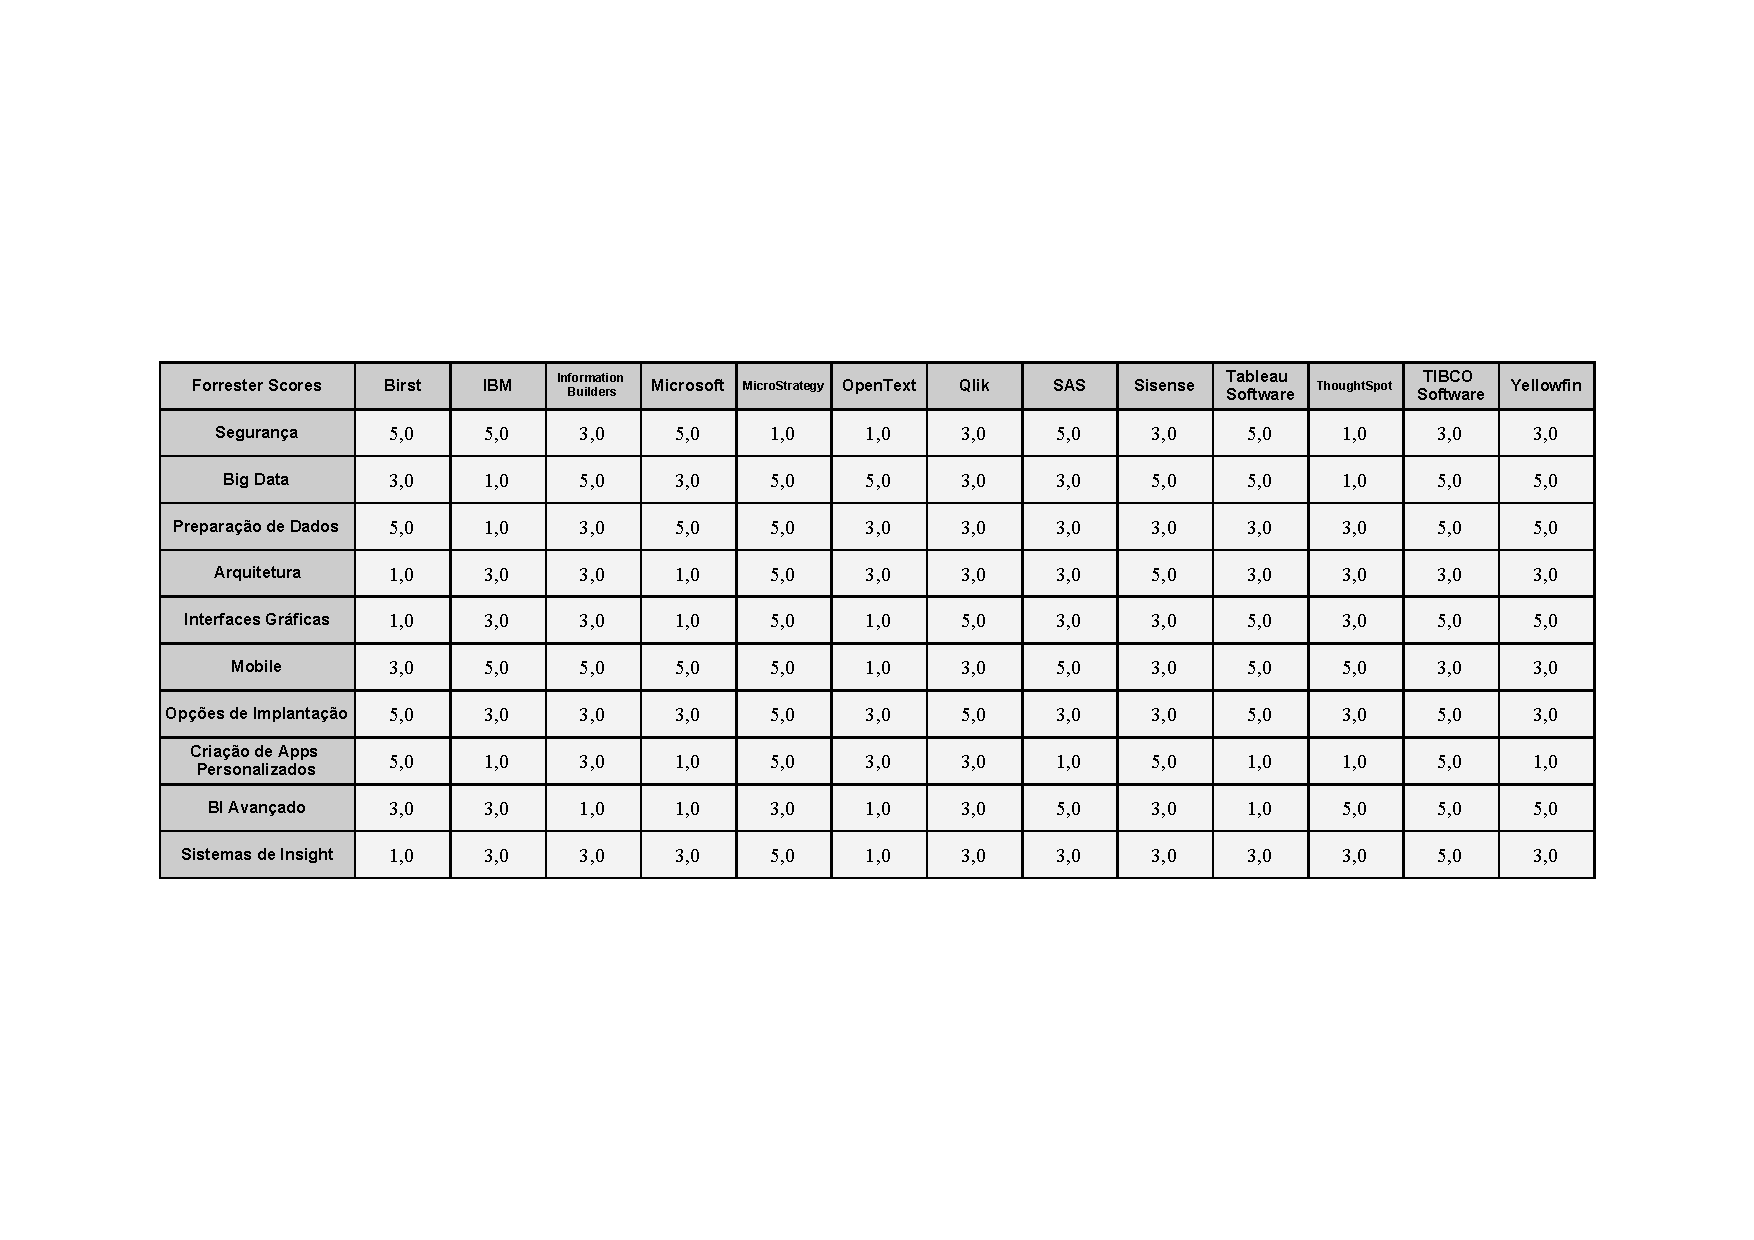
\includepdf[pages=-,angle=90]{forrester.pdf}
\end{landscape}
